%**************** Bilingual corpus building **************
\chapter{Compiling corpora for building data-driven prosodic models}
\label{chapter:corpusWorks}

In order to develop data-driven models related to speech prosody, one needs access to a sufficiently large corpus of speech samples that are annotated with prosodic features. Spoken samples collected to form a corpus serve for developing models for machine-learning applications as well as empirical research. A prosodically annotated spoken corpora usually consists of speech samples, their transcriptions and certain acoustic and prosodic labels associated with it. There is a few number of publicly available speech corpora that serve for prosody research as it is hard to process and annotate \citep{rosenberg}. One major work that this dissertation involves is collection of corpora to develop prosodic models on spoken language applications. This chapter presents: two prosodically annotated corpora that were used during this work, methodologies followed in compiling them and also further tools that were used and developed during the process.

There are two different methods for compiling spoken language corpora. First approach involves recording of designated speakers reading prepared text material in a controlled environment. Although this approach is the best way to obtain noiseless data, it is very expensive and hard to re-scale. Moreover, it poses a further disadvantage if prosody is an important aspect. As speakers are placed in a controlled environment their speech lacks the prosodic features that would normally be present in a more natural setting. 

Another approach to corpus development lies in exploiting readily available recorded material. This type of data is often called as found data and it includes any type of data that is available in public domain like audiobooks, public broadcast, conference talks. Material lying outside of public domain like copyrighted movies etc. can also be used within fair use principles. 

Using found data still implies some labour in development of various automated and manual processing methodologies to shape it to the need of the application need. One major disadvantage is the noise it introduces. On the other hand, two big advantages that it gives are that (1) the speakers can have more naturally expressive prosody, and (2) relatively low-cost scalability that comes with development of automated extraction methods. 

For the sake of obtaining data to be used in the methodologies presented in this dissertation, automated approaches that exploit readily recorded material were followed \citep{bucc, Oktem2018}. Two main sources of spoken data have taken advantage of: conference talks and subtitled movies and TV shows. The methodologies developed to process this material were compiled as open-source software libraries accessible online\footnote{\url{http://www.github.com/alpoktem}} (Sections \ref{corpusWorks:toolkit} and \ref{corpusWorks:movie2parallelDB}). Two corpora were obtained through the result of these processes: First one is the re-compiled and published \textit{TED talks corpus}, which is modified from \cite{Farrus:SP:2016} to suit experiments related to prosodic punctuation recovery task (Section \ref{corpusWorks:ted}). Second is the \textit{Heroes corpus}, which consists of parallel English and Spanish speech segments gathered from a TV series to suit prosodic translation task (Section \ref{corpusWorks:heroes}). Both of these corpora are made accessible openly through UPF Digital Repository\footnote{\url{repositori.upf.edu}}. 

Another task as important as obtaining of prosodically annotated corpora is analyzing them in terms of various prosodic features. The nature of prosodic data introduces its challenges and thus necessitates specialized tools to accommodate its analysis. In this chapter, I will also present \textit{Prosograph} \citep{prosograph}, which helps analyze data of this type in a simple and clear way (Section \ref{corpusWorks:prosograph}). 

\section{Toolkit for Prosodically Annotated Speech Data Creation}
\label{corpusWorks:toolkit}

In this section, I will introduce some of the principal tools employed which served an important role in the corpus development processes. 

\subsection*{Proscript for Prosodic Data Handling}
%Introduce the problem and need
Handling speech data together with prosodic annotations introduces its own challenges. Prosody can be seen as a phenomena parallel to the words uttered in speech. There has been considerable work on symbologies to represent prosodic aspects of speech together with its written form. For example, ToBI convention introduced in \cite{tobi} represents speech prosody in 4 tiers. These four tiers are agreed annotation styles for representing intonation, accents and breaks in correspondence with utterance. 

Computational applications that deal with prosody necessitate a standard in representing the structure of speech with its orthography and prosody together. One of the most popular of these conventions is the \textit{TextGrid} file format, which is used by \textit{Praat} \citep{boersma01}. This XML based file format stores any number of tiers that can be used to label prosodic features. Although very useful for visualization in Praat, this format is not designed to be functional for viewing and manipulating for itself. Every tier defines which event occurs at what time on its own and it is difficult to associate events that occur in parallel in different tiers. Also, for handling raw acoustic features, Praat uses different file formats. Due to this design, a complete prosodic-acoustic representation of a short utterance ends up being represented with a clutter of files. Other tools such as \cite{L06-1340, ProsodyPro} are also based on Praat and are only runnable through its interface. 

%What is introduced?
An optimal and standard data structuring was needed in this study for two reasons: for accommodating creation and storage of prosodic data and also for easy processing with machine learning applications. \textit{Proscript} framework was created to remedy for this deficit. It is both a data representation format and a specialized library for creation, manipulation, reading and writing of this sort of data. The name \textit{Proscript} is a portmanteau of the words \textit{prosody} and \textit{transcript}. It is seen as an enhanced way of representing a speech transcript. Instead of tiers, speech is represented with its features that occur in parallel at discrete bounded intervals. These bounded intervals can be words or a group of words that is called ``segments''. A segment can represent, for example, a prosodic phrase, a sentence or a group of sentences. Any type of feature can be stored within these boundaries. Be it acoustic features such as intonation, intensity or morphosyntactic features as part of speech or speaker tags. 

\begin{table}[th]
  
  \centering
  \begin{tabular}{>{\arraybackslash} m{0.25\linewidth} | >{\arraybackslash} m{0.6\linewidth} }
    \toprule
    \textbf{Feature} & \textbf{Details} \\
    \midrule
    word                         & as a token                                           \\
    id							 & unique word id				                        \\
    speaker id                   & unique speaker id                                    \\
    start time                   & start time of the word in an associated audio file   \\
    end time                     & end time of the word in an associated audio file     \\
    pause                        & coming before and after the word                     \\
    punctuation                  & coming before and after the word                     \\
    POS                          & part-of-speech                                       \\
    ToBI                         & ToBI label                                           \\
    mean F0                      & in Hertz and log-scaled (semitones)                   \\
    mean intensity               & in decibels and log-scaled                            \\
    F0 contour                   & as a list in Hertz or semitones                      \\
    intensity contour            & as a list in Hertz or log-scaled                      \\
    speech rate                  & in second per syllable            \\
    \bottomrule
  \end{tabular}
  \caption{Word-level information kept in an example Proscript format file.}
  \label{tab:proscript}
\end{table}

\textbf{Proscript file format} is based on the CSV file format. First line is the names of features that particular file stores and the following lines are the sequence of syntactic units together with the features that go parallel with them. See Table \ref{tab:proscript} for an example of parallel features stored in a Proscript file. In this particular example the linguistic units are defined as words. The set of features is determined by the application. For example, a configuration to keep only word-alignment information would keep words and their starting and ending times. 

A Proscript file can represent a short utterance as well as a whole dialog between two speakers. Dialog turns, for example, can be represented as segments with the speaker id tagged. Use is kept highly customizable through the library. 

\textbf{Proscript Python library} was developed in order to make creation, manipulation and annotation of Proscript files as easy as possible. It can be imported from a Python script to batch process transcripted speech files, annotate them with the desired features and output as files. Both word alignment and prosodic-acoustic tagging software (explained in following subsections) is accessible through the library. 

Proscript as python package is accessible online\footnote{\url{http://github.com/alpoktem/proscript}}. Guide and example scripts are provided in the repository on development. A ``Proscripter'' script is provided to obtain Proscript file from a audio file and its transcription. 

Proscript file format is used as the accepted format in the other software frameworks (Prosograph, punkProse, transProse) developed in this dissertation.

\subsection*{\textit{Montreal Forced Aligner} for Speech-to-text Alignment}
%Why alignment is needed?
Speech-to-text alignment is the process of determining boundary points of words and phonemes present in speech audio recordings defined by their text transcriptions. It proves to be essential for the work in this dissertation as it helps to align prosodic features in speech within their morphological boundaries. 

For this task, the open-source \textit{Montreal Forced Aligner (MFA)} \citep{mfa} is employed. Forced alignment process is built on an automatic speech recognition system and requires its own acoustic models and a pronunciation dictionary. Although pre-trained models for both English and Spanish is provided through the website of the tool\footnote{\url{montreal-forced-aligner.readthedocs.io/}}, Spanish pronunciation dictionary is not openly available. For this reason, a Spanish pronunciation dictionary has been created that uses the same phoneme set as MFA\footnote{Resource available in: \url{https://github.com/TalnUPF/phonetic_lexica}}. Vocabulary has been gathered from the open source spell checker tool \textit{ISpell}\footnote{\url{https://www.gnu.org/software/ispell/}}. Phonetic transcriptions of each word in this dictionary was obtained with \textit{TransDic} software \citep{Garrido2018}.

\subsection*{\textit{ProsodyTagger} for Prosodic Feature Annotation}
In order to augment speech data with acoustic-prosodic features \textit{ProsodyTagger} is used. \textit{ProsodyTagger} \citep{tagger} is a part of the \textit{Praat on the Web} service\footnote{\url{kristina.taln.upf.edu/praatupf}} \citep{praatontheweb} and was provided by its main author Dr. Mónica Domínguez for carrying out prosodic feature annotation task within the Proscript library. The tool is based on \textit{Praat} and simplifies the process of extracting mean F0 and intensity features in speech given its word-boundary information as a TextGrid file. See Figure \ref{corpusWorks:figure:pros_features} for an illustration of the prosodic features extracted for a speech utterance using this tool. 

\begin{figure}
\centering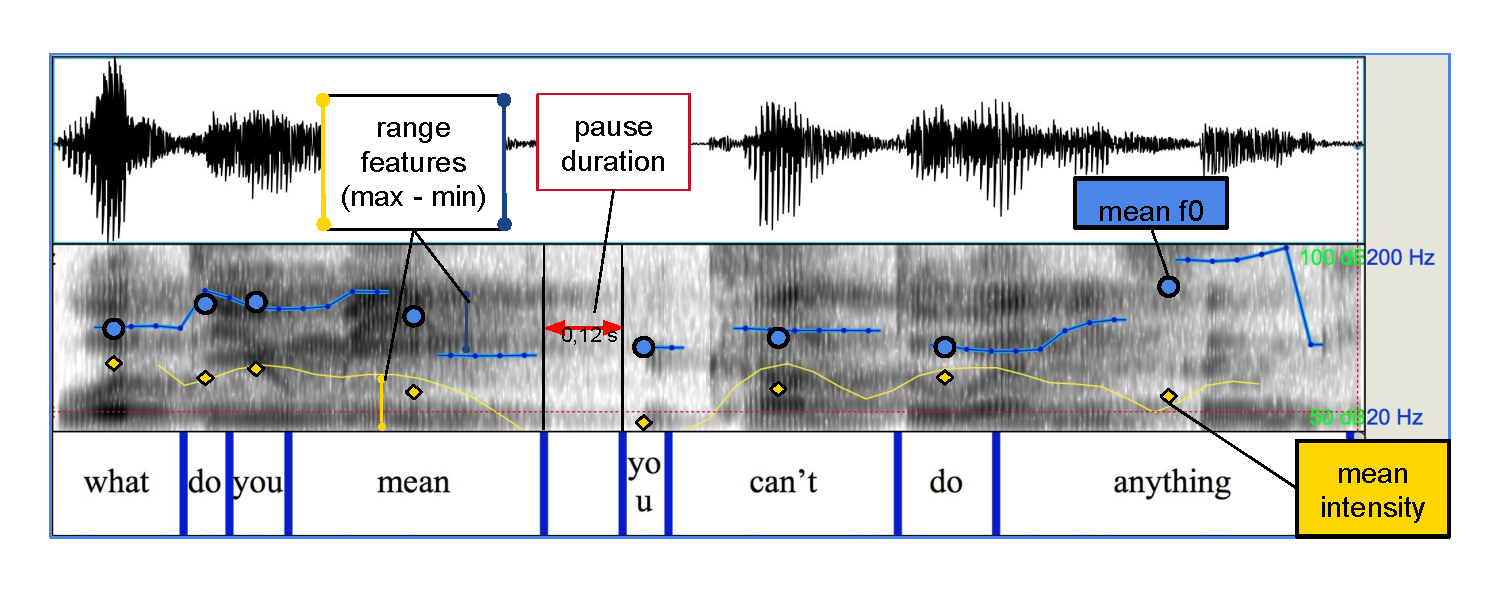
\includegraphics[width=\linewidth]{img/pros_features.pdf}
\caption{Word-level prosodic feature labelling.}
\label{corpusWorks:figure:pros_features}
\end{figure}

\section{Compiling the TED Talks Corpus}
\label{corpusWorks:ted}

In this section, I will introduce the TED talks corpus that was recompiled and published to serve for the automatic punctuation restoration work (explained in Chapter \ref{chapter:punkProse}). TED (Technology, Entertainment, Design) talks are a set of conference talks lasting in average 15 minutes each that have been held worldwide in more than 100 languages. They include a large variety of topics, from technology and design to science, culture and academia.  The corresponding transcripts, as well as audio and video files, are available openly on TED's website\footnote{\url{http://www.ted.com}}. For its public availability, TED talks have been the source of many corpora for linguistic analysis and machine learning-based applications. Different formats of corpora based on TED talks cover areas from automatic speech recognition \citep{tedlium} to document classification \citep{Hermann:2014:ACLphil} and machine translation \citep{cettoloEtAl:EAMT2012}. 

\cite{Farrus:SP:2016} studies paragraph-based prosodic cues in TED talks for the aim of improving naturalness in synthesizing spoken discourse. The dataset used for this work consists of 1365 talks published before 2014. Using the punctuation and paragraph annotated transcriptions available on the website, several prosodic analyses has been performed and stored at various lengths: words, sentences, segments (from subtitles) and paragraphs. Word and sentence timings were extracted using forced alignment. Pause durations between words were extracted from the provided word timings. Acoustic annotations are done at each interval automatically using Praat \citep{boersma01}. Fundamental frequency (F0) and intensity contours were extracted at 10 ms precision and then converted to semitones relative to speaker mean value. Thus, speaker mean values were represented by zero values in both cases. 

Although available on demand, this extensive corpus is not published in an open way. Moreover, it was found out that words, word timings, punctuation information and acoustic features associated with words were scattered among many files in the corpus. This made it difficult to process and create training data for machine learning based experiments. For these reasons, the corpus was re-processed, taking the information as it is, but making it easily readable. 

Due to some talks lacking acoustic annotations, the recompiled corpus consists of a subset of 1038 talks in the original corpus. These talks were given by 877 English speakers, which means that some speakers were present in various talks. Through counting of sentence-ending punctuation marks, 155174 sentences were calculated to be present in this version. The dataset is published online as \textit{Prosodically annotated TED talks}\footnote{\url{http://repositori.upf.edu/handle/10230/33981}} and is accessible through Attribution 4.0 International (CC BY 4.0) license\footnote{\url{https://creativecommons.org/licenses/by/4.0/}}. Source code used during the recompilation of this corpora is also provided online\footnote{\url{https://github.com/alpoktem/ted_preprocess}}.

\section{Automatic Extraction of Parallel Speech Corpora from Dubbed Movies}
\label{corpusWorks:movie2parallelDB}
Dubbing is the process of voice acting on top of the dialogues in a movie, TV series or documentary to make it accessible to viewers of another language. Popularity of dubbing of media material for a language depends greatly on the language culture of the country where the language is mainly spoken. For countries that prefer watching films in their mother-tongue, most movies and TV series go through this process before being released. Dubbing is carried out in professional studios and with professional voice actors. 

There are certain characteristics of art of dubbing that makes it an interesting candidate as a resource for parallel corpora. The process as a whole can be considered as a translation process. However, it has many more processes involved than just merely translating the movie script. One requirement it entails is that the voice-over recordings must match the lip movements of the actors. To ensure this, translations are made that match the length of actor lines and silenced segments within. Once a translation that fits a line is found, voice actors record the segment over the original movie respecting the way of acting of the original actors. It can be seen as a way of re-enactment of the line but with another language. Eventually, the voice-over doesn't only carry the content to the dubbing language but also the paralinguistic aspects that go with it. For example, if the original actor speaks in a particular tone (angry, sad, happy etc.), the dubbing artists also speak in the same tone. To match lip movements, they pause at the same points. Further remarks such as emphasis, irony, mockery are also expressed in a similar fashion within the general context of the scenario.  

A methodology has been built around getting advantage of this type of resource to obtain parallel speech corpora. In contrast with a methodology based on collecting samples in a controlled environment, I propose to exploit dubbed movies where expressive speech is readily available in multiple languages and their corresponding aligned scripts are easily accessible through subtitles. The time information in subtitles makes it easy to align sentences of different languages since timing is correlated to the audio. 

The proposed methodology needs only raw data, does not require any training (as is the case of previous work \citep{tsiartas2011bilingual}) and satisfies the following requirements: (1) it is easily expandable, (2) it supports language pair where dubbed material is available, (3) it can handle any domain and speech style, (4) it delivers a parallel spoken language corpus with annotated expressive speech which is present in movies, and (5) it doesn't violate the fair use principles that go with copyrighted material (see Section \ref{corpusWorks:fairuse}). This type of data proves to be valuable both for cross-lingual prosodic research and spoken machine translation with prosodic modelling. 

\subsection{Methodology}

\afterpage{%
    \begin{figure}[p]
      \centering
      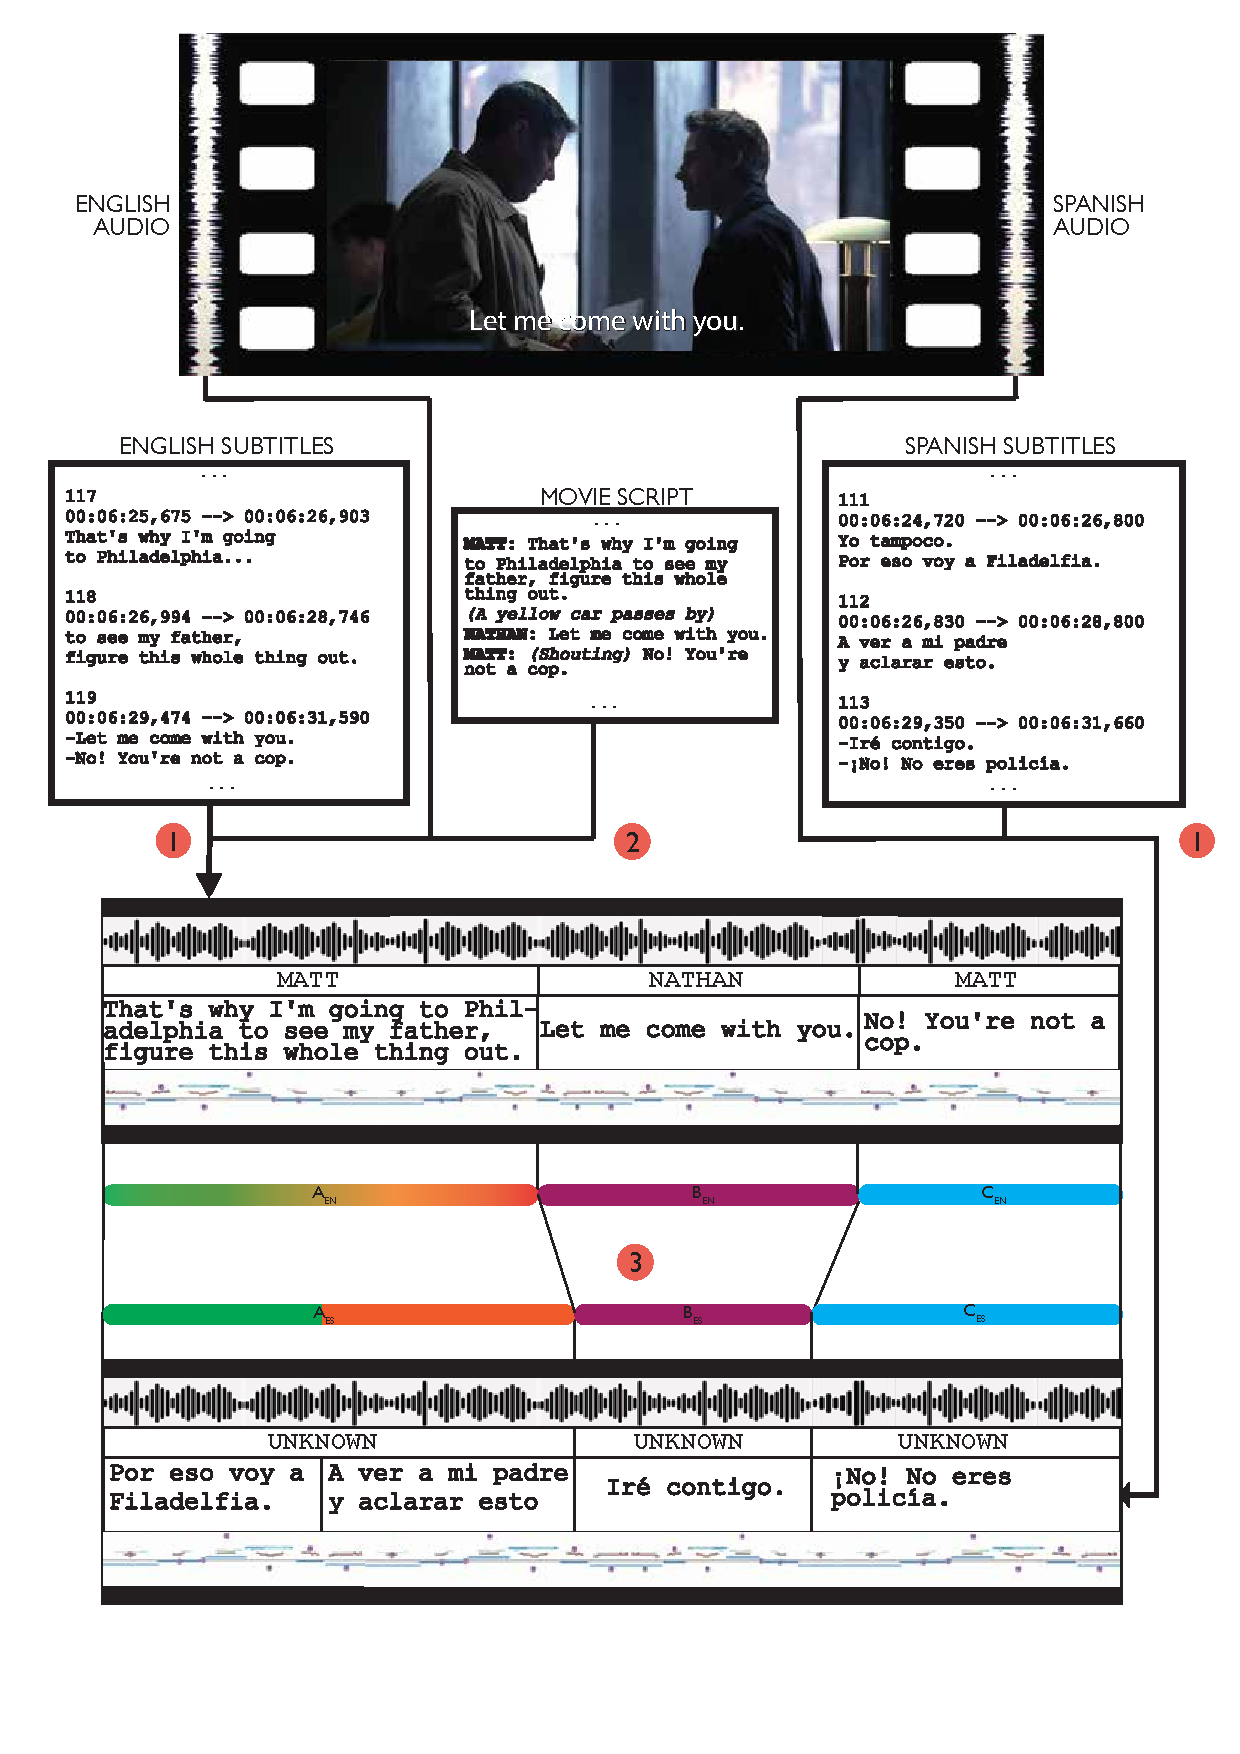
\includegraphics[width=\linewidth]{img/movie2parallelDB/movie2parallelDB-example_pipeline.pdf}
      \caption{Processes 1, 2 and 3 of the methodology illustrated on a portion of a movie. }
      \label{corpusWorks:fig:example_pipeline}
    \end{figure}
    \clearpage
}

% Explanation of the overall methodology. 
The methodology for obtaining a parallel corpus from a dubbed media consists of three stages: (1) a monolingual step, where audio+text pairs are extracted from the movie in both languages using transcripts and cues in subtitles, (2) paralinguistic feature annotation (speaker information and prosody) and (3) alignment of monolingual material to extract the bilingual segments. See Figure \ref{corpusWorks:fig:overall-scheme} for an overview of the system pipeline. Figure \ref{corpusWorks:fig:example_pipeline} further illustrates the whole process on an example portion of a movie. I will now explain each process in detail.

\begin{figure}[t]
  \centering
  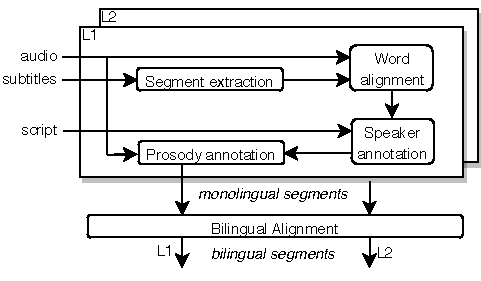
\includegraphics[width=0.6\linewidth]{img/movie2parallelDB/movie2parallelDB-pipeline.pdf}
  \caption[Overall parallel corpus extraction pipeline from movies.]{Overall corpus extraction pipeline. Audio excerpts are first processed in each language and then aligned to obtain bilingual segments.}
  \label{corpusWorks:fig:overall-scheme}
\end{figure}

\subsubsection*{Audio Segment Mining Using Subtitles}
Subtitles are the source for obtaining both (1) audio transcriptions, and (2) timing information related to utterances in a movie. These information are contained in a standard \textit{srt}\footnote{SubRip text file format \url{https://www.matroska.org/technical/specs/subtitles/srt.html}} subtitle file, entry by entry like the structure below:

\begin{lstlisting}
1
00:06:25,675 --> 00:06:26,903
That's why I'm going
to Philadelphia...
2
00:06:26,994 --> 00:06:28,746
to see my father,
figure this whole thing out.
3
00:06:29,474 --> 00:06:31,590
-Let me come with you.
-No! You're not a cop.
\end{lstlisting}

Each subtitle entry is represented by an index, time cues and the script being spoken at that time in the movie. The script portion can consist of single, multiple (\#3), or incomplete sentences (\#1). They can contain speech from single (\#1,2) or multiple speakers (\#3). Thus, using only these time cues does not suffice for extracting audio segments with complete sentences of a single speaker. To achieve this, word boundaries extracted with aligner software is combined with punctuation mark positions to split and merge segments as needed. Two entries are merged if the first one does not end with a sentence-ending punctuation mark and the second one starts with a lowercase letter. Multi-speaker segments were split from the words following speech-dashes [-]. This process is marked with the label "1" on Figure \ref{corpusWorks:fig:example_pipeline}.

The resulting segments from the subtitle excerpt from above would be:
\begin{enumerate}
    \item That's why I'm going to Philadelphia to see my father, figure this whole thing out.
    \item Let me come with you.
    \item No! You're not a cop.
\end{enumerate}

\subsubsection*{Speaker Annotation Through Scripts}
Movie scripts, which contain dialogue and scene information, are valuable pieces of information for determining the segment speaker labels. Scripts follow approximately the same format: Actor/actress name is followed by the line they say. In between, there might be non-spoken information in brackets. An example excerpt from a movie script is given below:

\begin{lstlisting}
MATT:   That's why I'm going to Philadelphia to see my father, 
        figure this whole thing out.
        (A yellow car passes by)
NATHAN: Let me come with you.
MATT:   (Shouting) No! You're not a cop.
\end{lstlisting}

Unlike subtitles, scripts do not have timing information. In order to map subtitle segments with the speaker information, an automatic procedure is followed. First, all non-spoken text included in brackets is removed. Then, speaker tags and corresponding lines are extracted with regular expressions depending on the format of the script. Next, segments coming from subtitles are mapped one by one to lines in the script. If 70\% of the words in a subtitle segment is included in a script turn, then the segment is labeled with the speaker of that turn. If it doesn't, up to five next script turns are checked as candidates. 

It should be noted that scripts are usually only available in the original language. However, since segments are aligned on a later step with their dubbed matches, they can share the speaker labels. In Figure \ref{corpusWorks:fig:example_pipeline}, speaker labels are extracted from the English script and matched with the subtitles. Spanish segments are left with an "UNKNOWN" label until they are aligned with their English matches. 

\subsubsection*{Word-level Acoustic Feature Annotation}

Each word in the extracted segments is automatically annotated with the following acoustic features: mean fundamental frequency (F0), mean intensity, speech rate and duration of non-voiced intervals (pauses) coming before and after. The first two features are extracted with \textit{ProsodyTagger}. Pause information is calculated from word-boundary information and speech rate is calculated using:

\begin{equation}
  \textit{word speech rate} = {\dfrac{\textit{\# syllables in word}}{\textit{word duration}}}
  \label{sprate}
\end{equation}

To represent speaker independent, perceptual acoustic variations in the segments, both F0 and intensity values are converted into logarithmic semitone scale relative to the speaker norm value. Thus, speaker mean values were represented by zero values in both cases. Semitone values are calculated with the corresponding formula:

\begin{equation}
  \textit{semitone}(x, \textit{norm}) = 12 * \log (\dfrac{x}{\textit{norm}})
  \label{semitone}
\end{equation}

The prosodic annotations are shown under the extracted segments with Prosograph feature visualizations in Figure \ref{corpusWorks:fig:example_pipeline}.

\subsubsection*{Cross-lingual Segment Alignment Based on Subtitle Cues}
\label{subsec:alignment}
The first three methodologies presented in this section dealt with extraction of segments in each language. This subsection explains how these segments are aligned to create the bilingual segment pairs. 

As explained earlier, the dialogues in the original and dubbed language correspond to each other time-wise. So, in order to align segments extracted for each language, timing information of the segments can be exploited. However, as subtitles show slight differences, alignment cannot be performed one-to-one. Also, the number of segments extracted in previous steps can differ for each language. This means that the segment alignments can be one-to-one, one-to-many, many-to-one or many-to-many depending on the sentencing structure in the subtitles. 

In order to create an alignment algorithm based on time cues, a metric is defined that measures the correlation percentage between two sets of ordered segments $\langle S_1, ...,  S_K\rangle$ and $\langle E_1, ...,  E_N\rangle$:
\begin{equation}
    \textit{correlation}(E_x, S_y) = \max(0,\dfrac{\textit{correlating}}{\textit{span}} \times 100)
\end{equation}
\begin{equation}
    \textit{correlating}(E_x, S_y) = \min(E_x^e, S_y^e) - \max(E_x^s, S_y^s)
\end{equation}
\begin{equation}
    \textit{span}(E_x, S_y) = \max(E_x^e, S_y^e) - \min(E_x^s, S_y^s)
\end{equation}

where $E_x^s$ and $E_x^e$ denote the starting and ending time of the $x^{th}$ English segment, $S_y^s$ and $S_y^e$ denote the starting and ending time of the $y^{th}$ Spanish segment. 

The alignment procedure is as follows. First, segments in both languages are checked one by one from beginning if they correlate more than the $T_{Sure}$ threshold. If they do, they are assigned as a one-to-one matched pair. If not, the possibilities of one-to-many, many-to-one or many-to-many matches are considered. This is done through computing the correlations between combinations of the current and two following segments and selecting the most correlating segment set pair. While considering combinations of the segments it is made sure that two merged segments belong to the same speaker and are not more than 10 seconds far from each other. If the combined segment set pair with highest correlation has a correlation of more than $T_{Merged}$ threshold, then the combinations are merged into one segment and paired with each other. 

Although the $T_{Sure}$ threshold catches most of the one-to-one mapping segments, many of them still fall below this threshold even if they map. So, another decision step is added where if one-to-one mapping correlation scores higher than merged pairings and it scores above a $T_{OK}$ threshold, then it is preferred as a matched pair. 

Figure \ref{corpusWorks:fig:example_pipeline} illustrates two examples of segment matching. First two Spanish segments are merged to align with the first English segment. Following segments are aligned one-to-one as their durations correlate enough.

After the matchings are done, if one of the languages have a speaker id labeled, it is copied to its matching segment. In Figure \ref{corpusWorks:fig:example_pipeline}, speaker information is copied from English segments to the Spanish segments. 

\subsection{Using the Parallel Corpus Extraction Framework}
This methodology is developed as a open source framework called \textit{movie2parallelDB} and is accessible online\footnote{\url{http://github.com/alpoktem/movie2parallelDB}}. The usage instructions are included in the online repository. 

The scripts are run with audio and their corresponding subtitles. Therefore, audio tracks needs to be extracted from the respective video prior to the process. Matching subtitles also needs to be acquired. 

One challenge that this method poses is that although it is easy to find subtitles in both original and dubbed languages of a movie, dubbing script might differ from subtitles. This is due to the difference in process between subtitling and dubbing. As it is mandatory to obtain exact transcription of the audio segments, subtitles need to be corrected prior to the process if this is the case. 

\subsection{Fair Use of Copyrighted Material}
\label{corpusWorks:fairuse}

Generally, material such as movie and TV shows are protected with copyright laws and limit the amount of its usage. This is governed by the principles of \textit{fair use}. It lets the use of copyrighted material for transformative and non-commercial purpose. The boundaries of what counts as transformative is not defined in a rigid way, but governed with guidelines and court decisions. The term ``fair use'' is originally defined by the United States law\footnote{\url{https://www.copyright.gov/fair-use/more-info.html}} and is influenced in other countries. United Kingdom, for example, allows non-commercial research on any material as long as it is within lawful access\footnote{\url{https://www.gov.uk/guidance/exceptions-to-copyright}}. 

The work introduced here assumes the work of collecting small portions of audio which cannot be reconstructed back to its original form for research purposes. The copyright on the original source of the segments has to be stated in both any publication explaining the work and during its access.

\section{Compiling the Heroes Corpus}
\label{corpusWorks:heroes}
The methodology presented in the previous section was put into practice by compiling a corpus from 2000's popular science fiction TV series \textit{Heroes}\footnote{Produced by Tailwind Productions, NBC Universal Television Studio (2006-2007) and Universal Media Studios (2007-2010)}. Originating from United States, Heroes ran in TV channels worldwide between the years 2006 and 2010. The whole series consists of 4 seasons and 77 episodes and is dubbed into many languages including Spanish, Portuguese, French and Catalan. Each episode runs for a length of 42 minutes in average. 

\subsubsection*{Raw Data Acquisition}
The DVD's of the series were obtained from the Pompeu Fabra University Library. Episodes were extracted using the \textit{Handbrake} software and were saved as \textit{Matroska format (mkv)} files. Mkv files can hold multiple channels of audios and subtitles embedded in it like DVDs. In order to run \textit{movie2parallelDB} scripts, audio and subtitle pairs for both languages needed to be extracted. Audio was extracted using the \textit{mkvextract} command line tool\footnote{\url{https://mkvtoolnix.download/}}. As subtitles were embedded as bitmap images in the DVD, an optical character recognition (OCR) software\footnote{Through a functionality provided by Subler: \url{https://subler.org/}} was used to convert them to \textit{srt} format subtitles. As OCR is an error-prone process, the resulting srt files needed to be spell checked. 

In total, 21 episodes were processed to obtain 25 hours English and Spanish audio with their corresponding subtitles. The episode scripts were obtained from a fan web page\footnote{\url{https://heroes-transcripts.blogspot.com/}}. 

\subsubsection*{Manual Subtitle Correction Work}
The Spanish subtitles needed slight correction in order to match the Spanish audio. It was observed that the Spanish subtitle transcripts were matching the Spanish audio in approximately 80\% of the cases. As exact correspondence between audio and transcription was aimed, a correction process was carried out. Both subtitle transcripts and time-stamps had to be corrected to match exactly what is being spoken on the dubbing audio and when. This process was done using a subtitle editing program \textit{Aegisub}\footnote{\url{http://www.aegisub.org/}}. 

An advantage the manual correction process gives is the opportunity to filter out unwanted audio portions that would otherwise end up in the corpus. This process is necessary especially in the case the source material is noisy. During the correction process, subtitle segments that contained noise and music, overlapping or unintelligible speech and speech in other languages (e.g.~Japanese) were removed. The spell checking and timestamps and script correction of 21 episodes was done by two annotators and took 60 hours in total. 

For each episode to be processed, the annotators were provided with the episode video, English and Spanish subtitles extracted with the OCR software. The correction procedures for each episode were as follows:
\begin{enumerate}
    \item Automated correction of OCR errors in English subtitles.
    \item Manual correction of English subtitles with a spell checker.
    \item Automated correction of OCR errors in Spanish subtitles.
    \item Manual correction of Spanish subtitles with a spell checker.
    \item Proofing and correction of the Spanish subtitles.
\end{enumerate}

The automated correction process involved a basic substitution procedure for the character errors that the OCR software did consistently. For example the letter `ñ' would be mistaken almost always as `fi' or `I's would be mistaken as lowercase `L's. For further non-standard errors, the spell checker provided in \textit{Aegisub} software was employed. Each spelling mistake in the subtitles were replaced with its corrected version.

\begin{table}[]
\begin{tabular}{|>{\arraybackslash} m{0.48\linewidth} | >{\arraybackslash} m{0.48\linewidth} |}
\hline
\textbf{Subtitle Entry} & \textbf{Audio Transcript}           \\
\hline
\begin{tabular}[c]{@{}l@{}}-Te presento a tu compañero.\\ -¿Me vas a cambiar?\end{tabular} & \begin{tabular}[c]{@{}l@{}}-Te presento a tu compañero.\\ -¿Me cambiar\'as?\end{tabular} \\
\hline
Me han tenido dos años, pensar\'an que los abandoné. & Me han tenido encerrado dos años, pensaran que los abandoné.    \\
\hline
Discutimos,...   & Empezamos a discutir...  \\
\hline
\begin{tabular}[c]{@{}l@{}}-Nunca quise...\\ -Cierra la boca! Escucha.\end{tabular} & \begin{tabular}[c]{@{}l@{}}-Yo nunca quise...\\ -Cierra la boca! Escucha.\end{tabular} \\
\hline
Hablaremos cuando vuelva, ¿vale? & Hablaremos mas cuando vuelva, ¿vale? \\
\hline
\end{tabular}
\caption{\label{corpusWorks:table:heroes_proofing}A selection of non-matching subtitle entries and dubbing scripts in Heroes series episodes.}
\end{table}

Last step involves checking of the transcripts and timings of each entry in the Spanish subtitles. Entries that do not correspond to the speech in the dubbed audio were corrected. Also, start and end time of the subtitle entries were adjusted so that it fits perfectly to the spoken segment. See Table \ref{corpusWorks:table:heroes_proofing} for a selection of entries that showed difference in transcript between subtitle entries and dubbing transcript. Depending on the episode, about 10\% to 20\% of the subtitle transcript needed to be corrected for minor differences. 

\subsubsection*{Heroes Corpus in Numbers}

Statistics of the first preparation sprint of \textit{The Heroes Corpus} are presented in this section. 21 episodes from season 2 and season 3 were processed. Total audio durations of 7000 parallel segments is about 9.5 hours (see Table \ref{tab:duration}). Counts of several linguistic units (words,tokens, sentences) in the final parallel corpus are presented in Table \ref{tab:counts}. Tokens represent words plus punctuation marks. A summary of how much of the content in one episode ended up in the dataset in average is presented in Table \ref{tab:episode}.  

\begin{table}[ht]
\centering
\begin{tabular}{lcc}
\toprule
 & \textbf{English} & \textbf{Spanish}\\ \midrule
{Total duration} &  4:45:36 & 4:43:20 \\
{Avg. duration/segment} & 00:02.44 & 00:02.42 \\\bottomrule
\end{tabular}
\caption{\label{tab:duration} Heroes corpus duration information.}
\end{table}

\vspace{5mm}

\begin{table}[ht]
\centering
\vspace{4mm}
\begin{tabular}{lcc}
\toprule
 \textbf{Counts}             & \textbf{English} & \textbf{Spanish} \\ \midrule
{\# words}                  & $56\,320$ & $48\,593$  \\
{\# tokens}                 & $72\,565$ & $63\,014$ \\
{\# sentences}              & $9\,892$  & $9\,397$ \\ 
{Avg. \# words/sentence}    & $5.69$    & $5.17$ \\ 
{Avg. \# words/segment}     & $8.04$    & $6.94$ \\ 
{Avg. \# sentences/segment} & $1.41$    & $1.34$ \\ \bottomrule
\end{tabular}
\caption{\label{tab:counts}Word, token, sentence counts and average word count for parallel English and Spanish segments.}

\end{table}



\begin{table}[ht]
\centering
\begin{tabular}{lcc}
\toprule
 \textbf{Counts} & \textbf{English} & \textbf{Spanish} \\  \midrule
{Avg. \# sentences (subtitles)} &  $647$ & $554$  \\
{Avg. \# sentences (extracted)} & $628$ & $513$ \\
{Avg. \# segments} & $526$ & $459$ \\
{Avg. \# parallel segments} & \multicolumn{2}{c}{$334$}\\
\bottomrule
\end{tabular}
\caption{\label{tab:episode}Averages numbers for each episode. }
% \toni{I would have used absolute numbers (not by episode), as these are more easily compared with table 3.3 and 3.4}
\vspace{-6mm}
\end{table}

\subsection*{Discussion}
The first version of the Heroes corpus shows that the proposed methodology for bilingual corpus building is successful in terms of the quality of the segments extracted. Correct alignment of segments and audio-transcription match was evaluated manually on selected samples. Although no thorough analysis has been followed, it shows that in general the parallel segments were well detected. 

The Spanish subtitle correction task was the only time-consuming part of the whole process. However, the task showed its usefulness for obtaining clean parallel segments. Subtitle segments that were removed during the correction process ensured the elimination of unwanted audio portions. 

Table \ref{tab:episode} shows the amount of information loss at various stages. The first one being the segment mining process where in average 5\% of the sentences are lost due to the word segmentation skipping noisy speech. The difference in number of segments and sentences is that segments can consist of merged sentences. The biggest loss happens at the stage of cross-lingual segment alignment where in average 30\% of the segments in each language are left unmatched. This percentage is directly affected by the alignment parameters explained in Section \ref{corpusWorks:movie2parallelDB}. For example, selecting a lower $T_{Sure}$ leads to detection of more aligned segments but also to more mismatches. A similar logic applies to $T_{OK}$. Choosing a lower $T_{Merged}$ leads to a better coverage of the sentences but segments end up being longer and fewer this way. After experimenting with a handful of parameter combinations, this parameter combination proved to be the most optimal for this task: $T_{Sure} = 70 \%$, $T_{Merged} = 80 \%$ and $T_{OK} = 30 \%$.

\section{Prosograph for Aiding Study of Large Speech Corpora}
\label{corpusWorks:prosograph}
Prosody conveys several communication elements such as meaning, intention, and emotions, among others. Being able to clearly visualize the different elements involved in prosody --intonation, rhythm, and stress-- may be helpful for computational prosody research. Several speech analysis tools (e.g. Praat), together with derived scripts and tools \citep{ProsodyPro,mertens2004prosogram,praatontheweb} partially cover these needs by helping to visualize quantifiable speech features like fundamental frequency ($F0$) and intensity contours, word stress marking, or prosodic labeling. These tools work well when showing detailed analyses on data and visualizing one single utterance at a time, but fail in visualizing generalized word-averaged speech features of many utterances, e.g., a discourse or a collection of speech samples, at once.

\textit{Prosograph} was born from the need to study prosody of long segments of speech to see the relation of prosodic features with punctuation in text. Inspiration was taken from music scores and piano rolls that help reading and visualizing music. Similar to a musical analysis tool, Prosograph helps visualize acoustic and prosodic structure in speech together with its transcript. Also, through an interactive interface it makes it easy to listen to any portion of the displayed speech to accommodate auditory analysis \citep{prosograph}. 

\subsection{Implementation}

Prosograph is written in Python mode of Processing\footnote{\url{py.processing.org/}} because of its simplified programming of graphical and interactive features. In order to simulate music scores, the speech prosodic features are plotted in the vertical axis over a temporal horizontal axis. Words are put in order together with pauses and punctuation, and the prosodic features are drawn under each corresponding word. An overview of the tool can be seen in Figure \ref{corpus:figure:prosograph_dump}.

Two modes of Prosograph have been implemented: monolingual (standard) mode and bilingual mode. Bilingual mode makes it possible to view aligned parallel corpora. Aligned samples are displayed side by side to accommodate e.g. prosodic comparison. Figure \ref{corpus:figure:prosograph2_dump} illustrates an overview of Prosograph in bilingual mode. 

\begin{figure}
\centering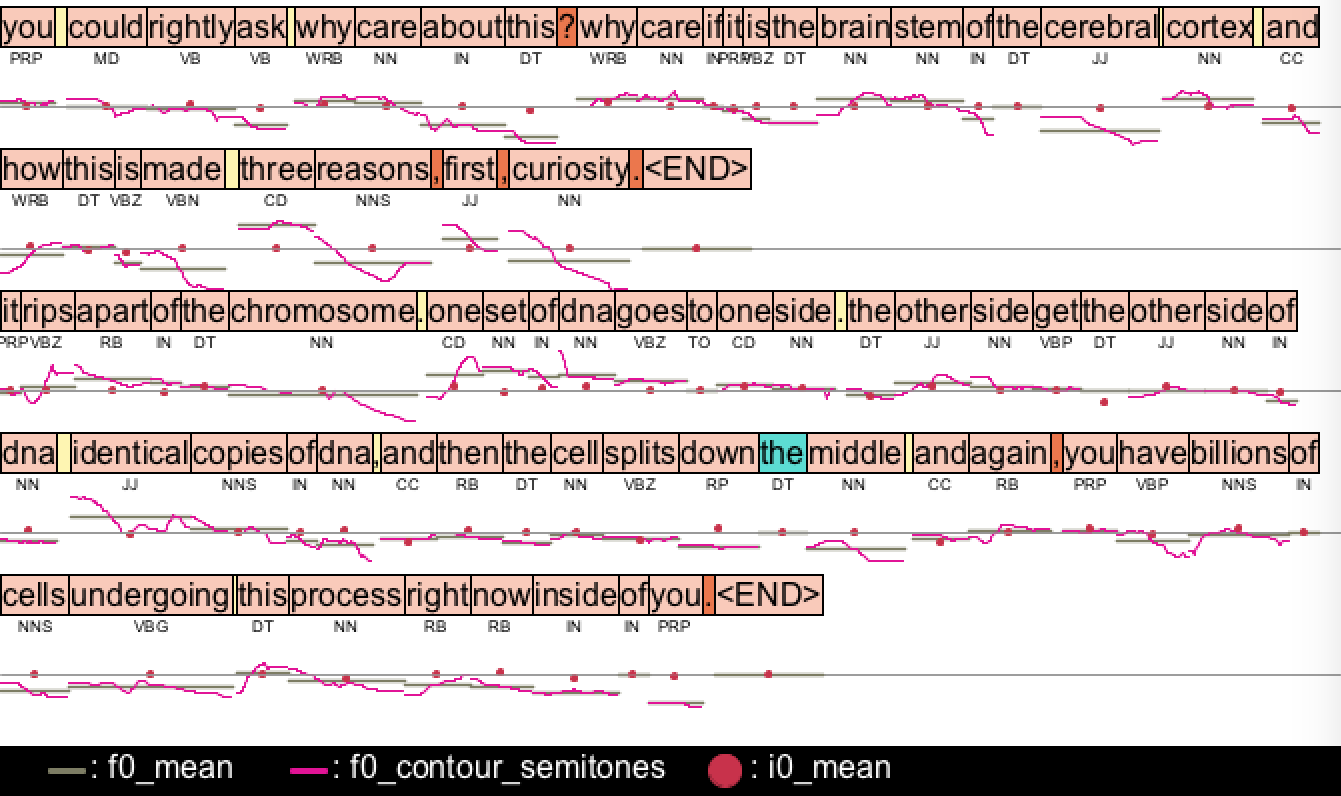
\includegraphics[width=\linewidth]{img/prosograph_dump_2.png}
\caption{An example of a visualization frame of segments from a conference talk with Prosograph.}
\label{corpus:figure:prosograph_dump}
\end{figure}

\begin{figure}
\centering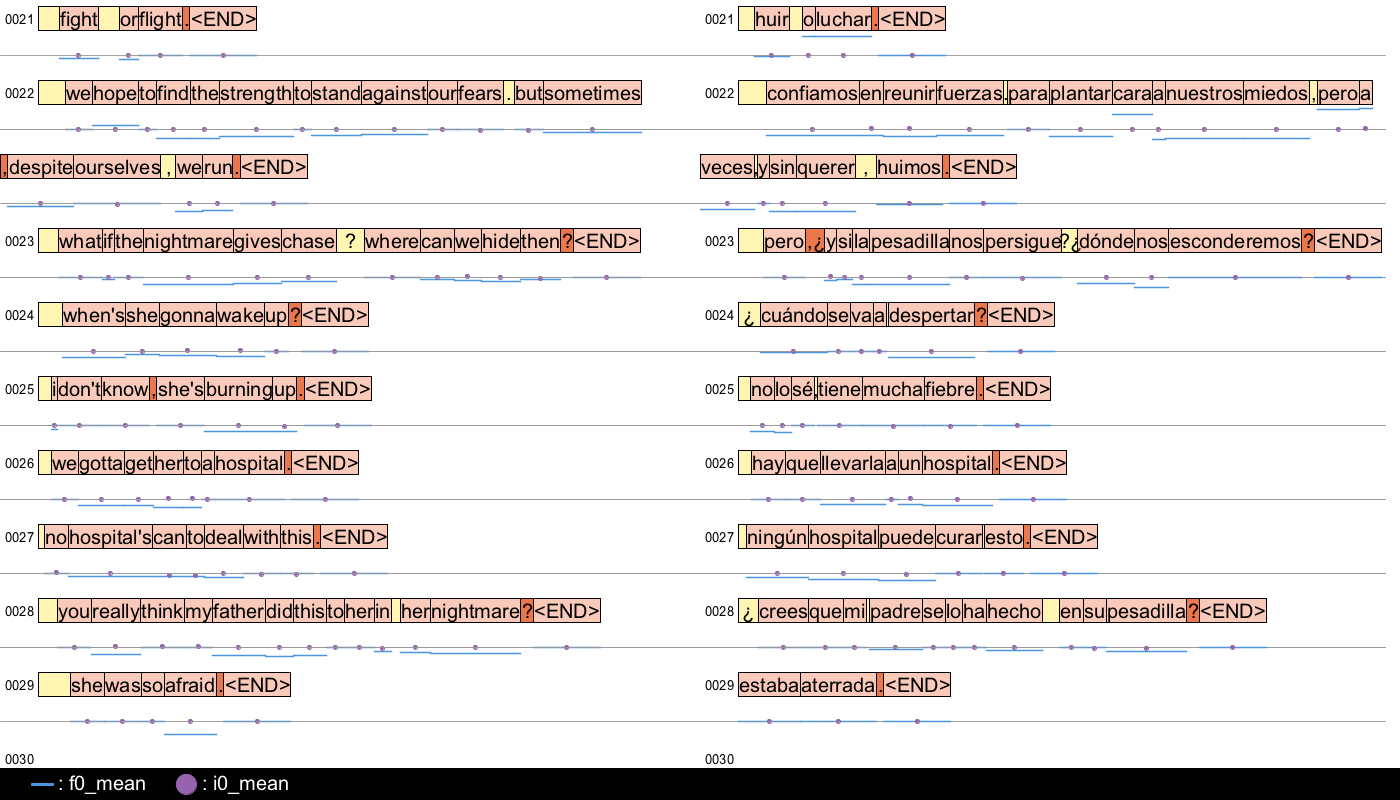
\includegraphics[width=\linewidth]{img/prosograph2_dump.png}
\caption{Visualizing parallel samples from an episode of Heroes Corpus with bilingual mode of Prosograph.}
\label{corpus:figure:prosograph2_dump}
\end{figure}

Prosograph reads prosodically annotated speech data from Proscript format files (see Section \ref{corpusWorks:toolkit}). Data path, and names and types of features in the files to be visualized is set in a configuration file before running the software. 

\subsection{Predetermined Feature Types}
Prosodic features differ in the way they encode words or sentences. For instance, word stress is a feature that represents salience among a group of words, intonation and intensity are continuous encodings throughout successive voiced phones, accent is a peak that occurs at a certain syllable in a word, etc. Because of these variations, each prosodic feature demands a special way for its storage and visualization. Prosograph allows the visualization of different kinds of prosodic features through the selection of its feature type in initialization. Predetermined feature types in Prosograph are listed below with some examples of prosodic features that they could be used for. Note that features are aligned to the words as they are in the Proscript format. 

\begin{itemize}
\item \textbf{pause-duration} holds the silence duration coming after the corresponding word. Paused intervals are visualized as an empty yellow box between words with a width proportional to the length of the pause (see Figure \ref{corpusWorks:fig:prosdatatypes}a).
\item \textbf{punctuation} holds the punctuation mark coming before or after the corresponding word. Punctuation marks are placed in the same axis with words. If a punctuation mark coincides with a pause, then it is placed inside the pause interval (see Figure \ref{corpusWorks:fig:prosdatatypes}b).
\item \textbf{binary-feature} holds a binary value determining if the corresponding word carries a certain feature (1) or not (0). This feature type can be used e.g. for word-stress. Bounding boxes of these words are drawn with a salient color (see Figure \ref{corpusWorks:fig:prosdatatypes}c).
\item \textbf{point-feature} holds a real numbered value that belongs to the corresponding word (e.g. standard F0 deviation, mean F0, median F0, etc.). It is placed at its value below the middle of the word's bounding box (see Figure \ref{corpusWorks:fig:prosdatatypes}d).
\item \textbf{line-feature} holds a real numbered value as point-features. They are visualized as a line below and parallel to the word. This feature type could be useful e.g. for visualizing better the mean F0 movement across the utterance (see Figure \ref{corpusWorks:fig:prosdatatypes}e).
\item \textbf{contour-feature} holds a sequence of value corresponding to a word. Each value is treated as curve bins and drawn as a line below the word in same length intervals. It is to be used e.g. for visualizing F0 curves or intensity curves or quantiles (see Figure \ref{corpusWorks:fig:prosdatatypes}f).
\item \textbf{percentage-feature} holds sequences of varying lengths where each value in the sequence corresponds to a percentage of time with respect to the duration of the word. A mark is placed at the corresponding time position below the word's bounding box. This feature type can be used e.g. to mark the point where the accent occurs in a word, F0 or intensity peaks (see Figure \ref{corpusWorks:fig:prosdatatypes}g).
\item \textbf{label-feature} holds a string label for their respective words. The label is written just below the respective word's bounding box. This feature type can be used to visualize prosodic labels such as ToBI or part of speech (see Figure \ref{corpusWorks:fig:prosdatatypes}h). 
\end{itemize}

\begin{figure}
\begin{tabular}{cc}
  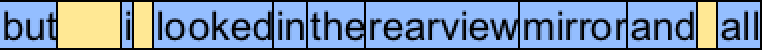
\includegraphics[height=4.5mm]{img/prosograph_datatypes/pause.png} &   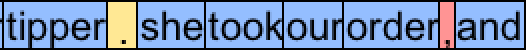
\includegraphics[height=4.5mm]{img/prosograph_datatypes/punctuation.png} \\
(a) pause-duration & (b) punctuation\\[6pt]
 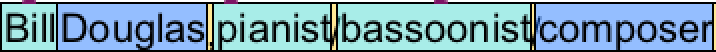
\includegraphics[height=4.5mm]{img/prosograph_datatypes/binary.png} &   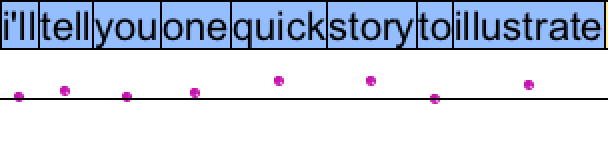
\includegraphics[height=11mm]{img/prosograph_datatypes/point.png} \\
(c) binary-feature & (d) point-feature\\[6pt]
 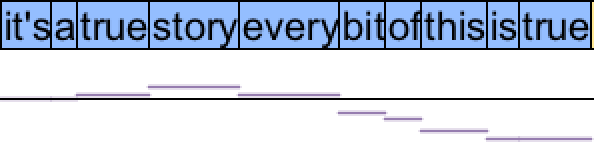
\includegraphics[height=11mm]{img/prosograph_datatypes/line.png} &   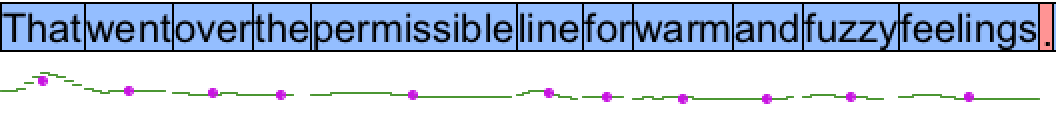
\includegraphics[height=8mm]{img/prosograph_datatypes/curve.png} \\
(e) line-feature & (f) contour-feature\\[6pt]
 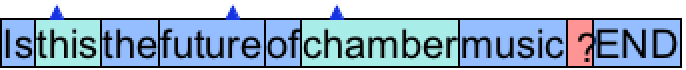
\includegraphics[height=6mm]{img/prosograph_datatypes/percentage.png} &   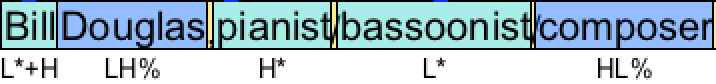
\includegraphics[height=7mm]{img/prosograph_datatypes/label.png} \\
(g) percentage-feature & (h) label-feature \\[6pt]
\end{tabular}

\caption{Word-aligned feature data types in Prosograph.}
\label{corpusWorks:fig:prosdatatypes}
\end{figure}

\subsection{Access and Usage}
Prosograph is made publicly available as an open-source software\footnote{\url{http://github.com/alpoktem/Prosograph}} under the GNU General Public License\footnote{\url{http://www.gnu.org/licenses/gpl.html}}. 

Once it is installed and the configurations are set, utterances in the dataset are shown in batches and user can navigate over the batches using keyboard shortcuts N(next) and B(previous). The current batch frame can be saved as an image by pressing S. 

%\toni{Just a comment: what a curious design that the colors are random at run-time!}

By default, colors of different prosodic features are set randomly at run-time. A legend showing which color belongs to which feature is shown at the bottom of the screen. If not easily distinguishable, the colors can be changed (again randomly) by pressing C on keyboard. 

To listen to a particular sample, beginning and end word of the utterance need to be selected. When P key is pressed, the utterance is played between the selected word interval. This is made possible if an audio file accompanies the Proscript file in the same directory with the same name. 

\subsection{Discussion}

Prosograph can be used for the analysis of prosodic features and patterns in a speech corpus. It has been designed to be robust for handling different types of prosodic data annotated on word level. By simplifying the process of observation and comparison of prosody, this application can be used in many areas of research such as language learning and acquisition, comparative studies in different languages, tone languages, audiovisual prosody, etc.

Prosograph was first implemented to aid feature selection process in the punctuation restoration methodology that this dissertation presents in Chapter \ref{chapter:punkProse}. After its development, it was used to demonstrate the results of this system and to reason how a neural punctuation restoration system behaves with respect to various prosodic features. Through the development of the bilingual mode, it proved its use in studying prosodic transformations in the dubbed translations in the Heroes corpus and helped inspire the prosodically enhanced translation system that is to be presented in Chapter \ref{chapter:transProse}. Also, with its easy integration with Proscript library, it simplifies creation of visualizations of speech samples for linguistic study. Visualizations of speech samples in this dissertation are also made with Prosograph. 

It should be noted that Prosograph is not a program that obligates its usage ``as-it-is''. It is a framework, written in a highly visual and simple programming language to be customized to the needs of its user. For instance, a linguist wanting to observe certain characteristics in a recorded corpus can set it up to display segments together with speaker information. The bilingual mode can be further extended to display utterances of two speakers together with a reference utterance and facilitate comparison. Another use-case could be real-time prosodic display and assessment for accent and intonation training. I hope the framework inspires researchers from different fields to study prosody and speech corpora in a visual and customizable way. 

\section{Conclusion}

In this chapter, I have introduced the data related work carried out to aid the machine learning-based methodologies that will be explained in the following chapters. The toolkits introduced include a library for the prosodic annotation and handling of segmented speech data, Proscript, a parallel corpus extraction framework, movie2parallelDB and a tool for the visualization of speech corpora, Prosograph. 

Two corpora that were prepared and packaged using these toolkits were also presented. These are: (1) TED talks corpus, which consists of prosodic annotations of TED conference talks and (2) Heroes corpus, which consists of prosodically annotated parallel speech segments from TV-movie domain. All of the resources developed are published openly for research purposes. 

In the next chapter, I will start with explaining the work carried out within the area of automatic transcription dealing with punctuation restoration. 
